\section{Page Directory Inspection Window}
The page directory inspection window allows you to inspect the page directory and its page tables. With the information provided by these windows you are able to translate a virtual address to the physical address.
\begin{figure}[H]
\begin{center}
	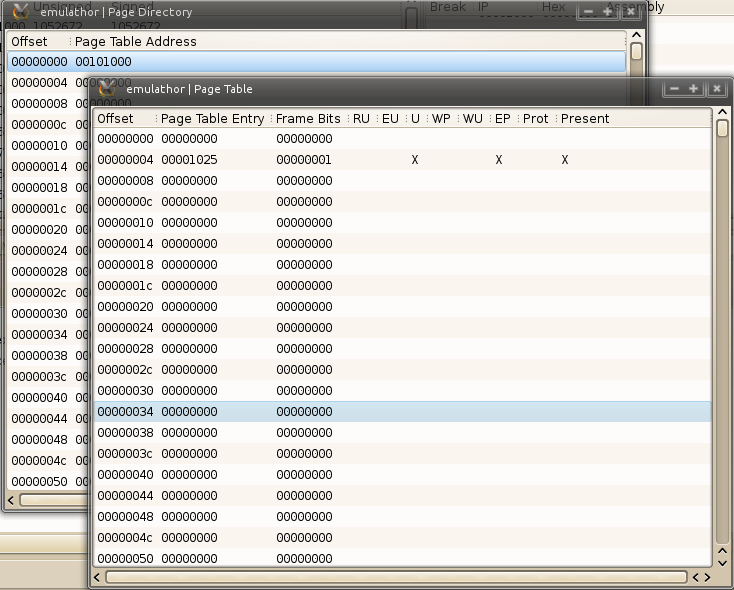
\includegraphics[width=0.5\textwidth]{./files/emu_gui_mmu.png}
\end{center}
	\caption{The page directory and page table inspection windows.}
\end{figure}

\subsection{Page Directory Inspection}
The page directory inspection window displays the content of the page directory. The offset corresponds to the page directory index of the virtual address. At this index resides the address of the page table. Double-click on a row to open the related page table in the page table inspection window.
\begin{figure}[H]
\begin{center}
	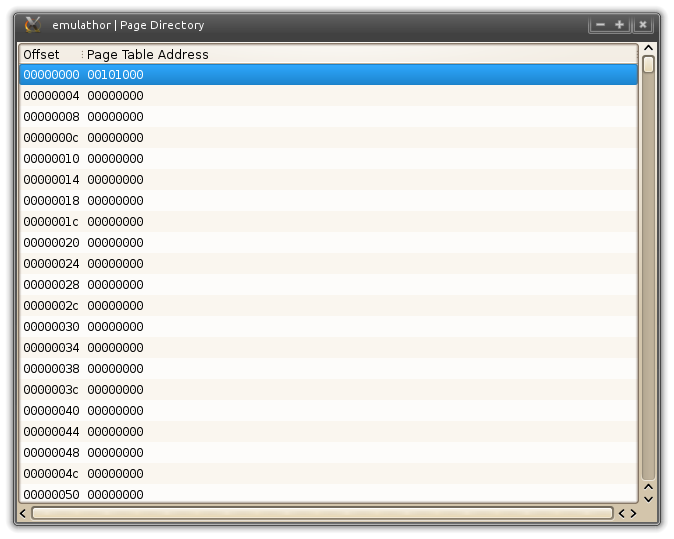
\includegraphics[width=0.8\textwidth]{./files/emu_gui_mmu_pagedir.png}
\end{center}
	\caption{The page directory with one page table set up.}
\end{figure}

\subsection{Page Table Inspection}
The page table inspection window shows the contents of a page table. Each row represents a page table entry. The columns have the following meaning:
\begin{description}
\item[offset] The page table index
\item[page table entry] The contents of the entry (including frame and control bits)
\item[frame bits] The frame bits of the physical address
\item[RU] Control bit: read-unprivileged
\item[EU] Control bit: executable unprivileged
\item[U] Control bit: used
\item[WP] Control bit: write privileged
\item[WU] Control bit: write unprivileged
\item[EP] Control bit: executable privileged
\item[Prot] Control bit: protected
\item[Present] Control bit: present
\end{description}


\begin{figure}[H]
\begin{center}
	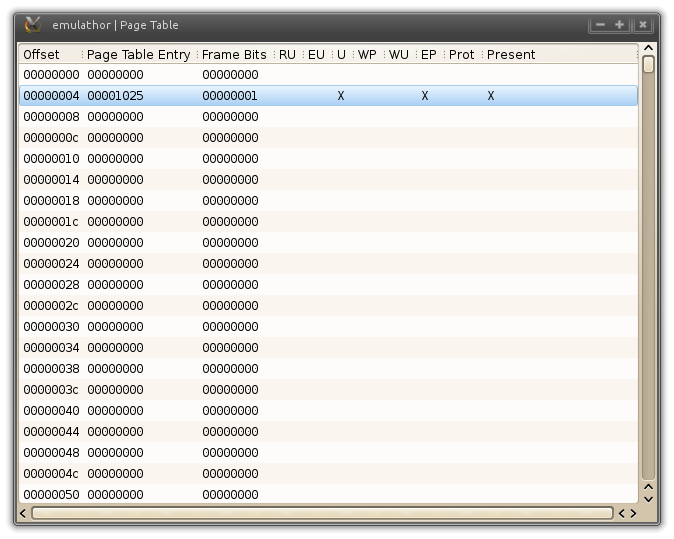
\includegraphics[width=0.8\textwidth]{./files/emu_gui_mmu_pagetable.png}
\end{center}
	\captionsetup{justification=centering}
	\caption{The page table entries with the first two pages \\mapped to the first two frames of the physical memory.}
\end{figure}
